\section{Authorization and Policy Enforcement}\label{sec:security-authZ}

Authorization in CFI-Care is decentralized, with the Backend-for-Frontend (BFF) acting as the primary enforcement point. 
It validates identity claims and enforces healthcare-specific access policies before requests reach the \ac{FHIR} server.

\subsection{BFF Middleware Pipeline}

The BFF implements a middleware chain for every protected route. 
This pipeline ensures that only validated requests with appropriate scopes are processed.

\begin{itemize}
    \item \textbf{JWT Integrity (JWKS):} The system utilizes the \texttt{jwks-rsa} and \texttt{jsonwebtoken} libraries to perform stateless verification of \acp{JWT}, where 
    signatures are validated against Keycloak's public keys fetched from the JWKS endpoint. 
    The middleware enforces strict checks on the issuer (\texttt{iss}), audience (\texttt{aud}), and the RS256 algorithm, with a configurable clock-skew tolerance.
    \item \textbf{Scope Pattern Matching:} The BFF parses the \texttt{scope} and \texttt{realm\_access} claims. It compares these against the required scopes. 
    \item \textbf{Identity Binding:} For patient-specific resources, the middleware enforces a binding check, ensuring the \texttt{patient} ID claim within the token matches the specific resource ID being requested in the URI.
    \item \textbf{Role-Based Access Context:} Access decisions to a patient's data are mediated through role checks and request-context middleware: patient-owned resources allow direct access, caregivers and practitioners require an active, non-expired grant with matching scopes. 
    Grant expiry is validated on every request by comparing the grant's stored timestamp.
    \item \textbf{Caller Restriction:} Administrative endpoints, such as the registration provisioning route, are restricted to a specific allow list of service clients.
\end{itemize}


The enforcement of this multi-tiered middleware hierarchy guarantees that malformed inputs or missing credential headers are caught.
This behavior was mapped via negative testing sequences \texttt{SEC-API-001} through \texttt{SEC-API-011}, proving structural verification resilience against forged tokens (see Section~\ref{sec:testing_results}).
Furthermore, live request manipulations intercepted via Burpsuite confirmed active perimeter isolation (Fig~\ref{fig:burp-cookie-auth})

\subsection{\texorpdfstring{\ac{CBAC}}{CBAC}}
Unlike role-based permissions which are stored in a central directory, a capability is a key that bundles the resource address and the permitted operations into a single unit stored in the system.
While RBAC is used for basic application navigation, the actual access to medical data is Capability-Based, 
% Meaning, holding a specific role isn't enough to access specific sources, a Capability must be obtained first, 
% for example the Consent \& Capability-based Access section \ref{sec:JIT} 
In this model, a Role acts only as a prerequisite for platform navigation; 
it does not authorize access to specific clinical resources, instead, 
access is mediated via the acquisition of an ephemeral Capability Token, 
as detailed in the JIT Consent protocol (Section \ref{sec:JIT})


\subsection{The \texorpdfstring{\ac{JIT}}{JIT} Consent Handshake Protocol}\label{sec:JIT}
\subsubsection{Concept: Separating Identity from Intent}

The JIT protocol enforces a strict Separation of Concerns: Keycloak handles Authentication (Identity Verification) and Role Mapping (RBAC), 
while the JIT logic handles context-specific Authorization (Intent Validation). 
This ensures that even a fully authenticated practitioner has -by default- zero access to clinical data until a Capability Token is issued by the patient after choosing the actions they consent to be executed on their data and for how long this token lasts.


% \ac{JIT} separates identity from intent, identity is established via an Identity Provider (Keycloak) using OpenID Connect, while Intent is localized, represented by a Capability Token stored in the system
% for example a doctor is authenticated on the system, and has an active Consent grant (Capability token) to access a patient's data
% the identity would be a registered doctor on the system with an active session issued by keycloak.
% the intent would be the doctor is authorized to see this patient's data for the time assigned at grant issuance.

% The protocol enforces a strict Separation of Concerns: Keycloak handles Authentication (Identity Verification), while the JIT logic handles Authorization (Intent Validation). 
% This ensures that even a fully authenticated practitioner has zero default access to patient data until a specific intent-based capability is issued through the handshake.


% CFI-Care separates Identity (who a user is) from Intent (what they are authorized to do in a specific context). 
% Identity is established via Keycloak (OIDC), while Intent is localized and ephemeral, represented by a Capability Token stored in the system. 
% This enforces a strict Separation of Concerns: Keycloak handles Authentication, while the JIT logic handles context-specific Authorization. 
% A practitioner, even if fully authenticated, possesses zero default access to patient data until a specific intent-based capability is issued through the handshake


\subsubsection{Technical Implementation}
\begin{itemize}
    % \item State Store: Redis set function's (function used to set a value in cache) `NX' is used for the \ac{OTP} to ensure idempotency by preventing the issuance of multiple conflicting active codes for a single patient session.
    \item Collision Avoidance: The \ac{OTP} issuance logic implements a recursive trial mechanism (up to 10 attempts) using Redis's SET command with the `NX' (Not eXists) option to guarantee the uniqueness of the 6-digit secret and prevent the issuance of multiple conflicting active codes for a single patient session.
    \item Notification: As soon as the requester for data access inputs the OTP in the field provided for them, a transient handshake ID is created and stored, meanwhile \ac{FCM} is used to push the request to the patient's device for real-time approval.
    \item Persistence: Once approved, the handshake ID is deleted from Redis and a grant is generated and stored.
    \item Identity Extraction: Access control is strictly enforced by extracting the \texttt{sub} claim containing the user's lengthy alphanumeric ID from the Keycloak-issued JWT, ensuring that users cannot spoof their identity in the request body
    % \item Audit Logging: Every transition triggers a logging event, capturing the IP, ID, HTTP action being performed on the data, and User-Agent for non-repudiation
    \item Scoped Capabilities: When a grant is issued, the system defaults to a restricted scope (patientID/*.read) unless specific scopes are specified, following the principle of least privilege
\end{itemize}

% \begin{center}
% \textbf{API Endpoints used for the protocol}
% \end{center}
% \begin{table}[H]
% \centering
% \renewcommand{\arraystretch}{1.3}
% \begin{tabular}{|l|l|p{4cm}|p{5cm}|}
% \hline
% \textbf{Endpoint} & \textbf{Actor} & \textbf{Request Body} & \textbf{Success Response} \\ \hline
% \texttt{POST /request-otp} & Patient & N/A (Uses JWT sub) & \{otp, expiresIn\} \\ \hline
% \texttt{POST /verify-otp} & Practitioner & \{otp\} & \{handshakeId, targetId\} \\ \hline
% \texttt{POST /grants} & Patient & \{handshakeId, approved, durationMinutes, scopes\} & \{message, grant\} \\ \hline
% \texttt{DELETE /grants/:id} & Patient & practitionerId (URL Param) & \{message: "Grant revoked"\} \\ \hline
% \end{tabular}
% \caption{API Specification for the JIT Consent Handshake Protocol}
% \label{tab:jit-api-spec}
% \end{table}

\subsection{API Specification and Control Endpoints}

To implement the JIT Consent Handshake Protocol and manage the complete lifecycle of temporary capability grants, 
the system exposes structured routers in the backend, listed in detail here \ref{tab:api-matrix}. 
These endpoints -like all API endpoints- are strictly protected by token verification middleware.

\begin{center}
\setlength{\tabcolsep}{4pt}
\begin{longtable}{|p{5cm}|p{2.2cm}|p{3.2cm}|p{3.9cm}|}
\caption{API Endpoints used for the protocol} \label{tab:api-matrix} \\
\hline
\textbf{Endpoint \& Method} & \textbf{Actor} & \textbf{Payload Parameters} & \textbf{Primary Action} \\ \hline
\endfirsthead
\multicolumn{4}{l}{\tablename~\thetable{} \textit{(continued)}} \\
\hline
\textbf{Endpoint \& Method} & \textbf{Actor} & \textbf{Payload Parameters} & \textbf{Primary Action} \\ \hline
\endhead

\hline
\multicolumn{4}{|r|}{\textit{Continued on next page}} \\ \hline
\endfoot

\hline
\endlastfoot

\hline
\multicolumn{4}{|l|}{\textbf{1. Just-In-Time Handshake Initiation \& Capability Grant creation}} \\ \hline
\texttt{POST /api/handshakes/} \newline \texttt{request-otp} & 
Patient & 
N/A (\ac{JWT} Derived) & 
Clears existing user sessions in cache, generates a unique 6-digit random token. \\ \hline

\texttt{POST /api/handshakes/} \newline \texttt{verify-practitioner}\newline\texttt{-otp} & 
Practitioner & 
\texttt{\{otp\}} & 
Links practitioner metadata to target patient identity in the pending cache. \\ \hline

\texttt{POST /api/handshakes/} \newline \texttt{verify-caregiver-otp} & 
Caregiver & 
\texttt{\{otp\}} & 
Links Caregiver metadata to target patient identity in the pending cache, adds a caregiver onboarding key to later dynamically map the role to the user when grant is approved \\ \hline

\texttt{POST /api/handshakes/} \newline \texttt{create-grant} & 
Patient & 
\texttt{\{handshakeId, approved, duration, scopes\}} & 
Clears pending states from the cache; issues and stores a capability token. \\ \hline

\texttt{GET /api/handshakes/} \newline \texttt{pending} & 
Patient & 
N/A (\ac{JWT} Derived) & 
Queries active transaction states, automatically prunes expired identifiers from list. \\ \hline

\texttt{GET /api/handshakes/} \newline \texttt{status/:handshakeId} & 
Practitioner \newline / Caregiver & 
\texttt{handshakeId} (Param) \newline \texttt{patientId} (Query) & 
Evaluates polling state transitions (Pending, Approved, or Expired). \\ \hline

\hline
\multicolumn{4}{|l|}{\textbf{2. Patient Access Delegation Control}} \\ \hline
\texttt{GET /api/patient-grants/} \newline \texttt{grants} & 
Patient & 
N/A (\ac{JWT} Derived) & 
Fetches active access requests, drops expired keys. \\ \hline

\texttt{DELETE /api/patient-grants/} \newline \texttt{grants/:practitionerId} & 
Patient & 
\texttt{practitionerId} (Param) & 
Terminates specified grant, records event to audit logs. \\ \hline

\texttt{DELETE /api/patient-grants/} \newline \texttt{caregivers/}\newline \texttt{:caregiverId} & 
Patient & 
\texttt{caregiverId} (Param) & 
Terminates specified grant, records event to audit logs, withdraws target user's caregiver role mapping if no patient attachments remain. \\ \hline

\hline
\multicolumn{4}{|l|}{\textbf{3. Delegatee Resource Directories}} \\ \hline
\texttt{GET /api/practitioner} \newline \texttt{-grants/my-patients} & 
Practitioner & 
N/A (\ac{JWT} Derived) & 
Queries active delegated profiles out of the \ac{FHIR} server, drops expired grants. \\ \hline

\texttt{GET /api/caregiver-grants/} \newline \texttt{my-patients} & 
Caregiver & 
N/A (\ac{JWT} Derived) & 
Queries active delegated profiles out of the \ac{FHIR} server, drops expired grants. \\ \hline

\hline
\multicolumn{4}{|l|}{\textbf{4. Out-of-Band Notification Registration}} \\ \hline
\texttt{POST api/FCM/} \newline \texttt{fcm-token} & 
Patient & 
\texttt{\{fcmToken\}} & 
Binds individual devices to matching user contexts in the backend. \\ \hline
\end{longtable}
\setlength{\tabcolsep}{6pt}
\end{center}
% \label{tab:api-matrix}

The structural logic governing OTP lifespans was evaluated across 15 unit tests (\texttt{HANDSHAKE-001} to \texttt{HANDSHAKE-014}), this automated verification proved that cross-patient transaction hijacking variants are successfully trapped and audited, these tests are described at section~\ref{sec:logical-sec-testing-coverage}.

\subsubsection{Atomic Handshake Protocol}
To ensure the integrity of the delegation process, the system implements a "Burn-on-Read" policy. 
The verification of the OTP is an atomic operation -as displayed in the following state diagram Figure~\ref{fig:consent-endpoints} highlighting operations used by each endpoint in the flow- where it's invalidated at the same moment as the verification operation, this eliminates the \ac{TOCTOU} race condition, it also eliminates the window of opportunity for replay attacks.


\begin{figure}[H]
    \centering
    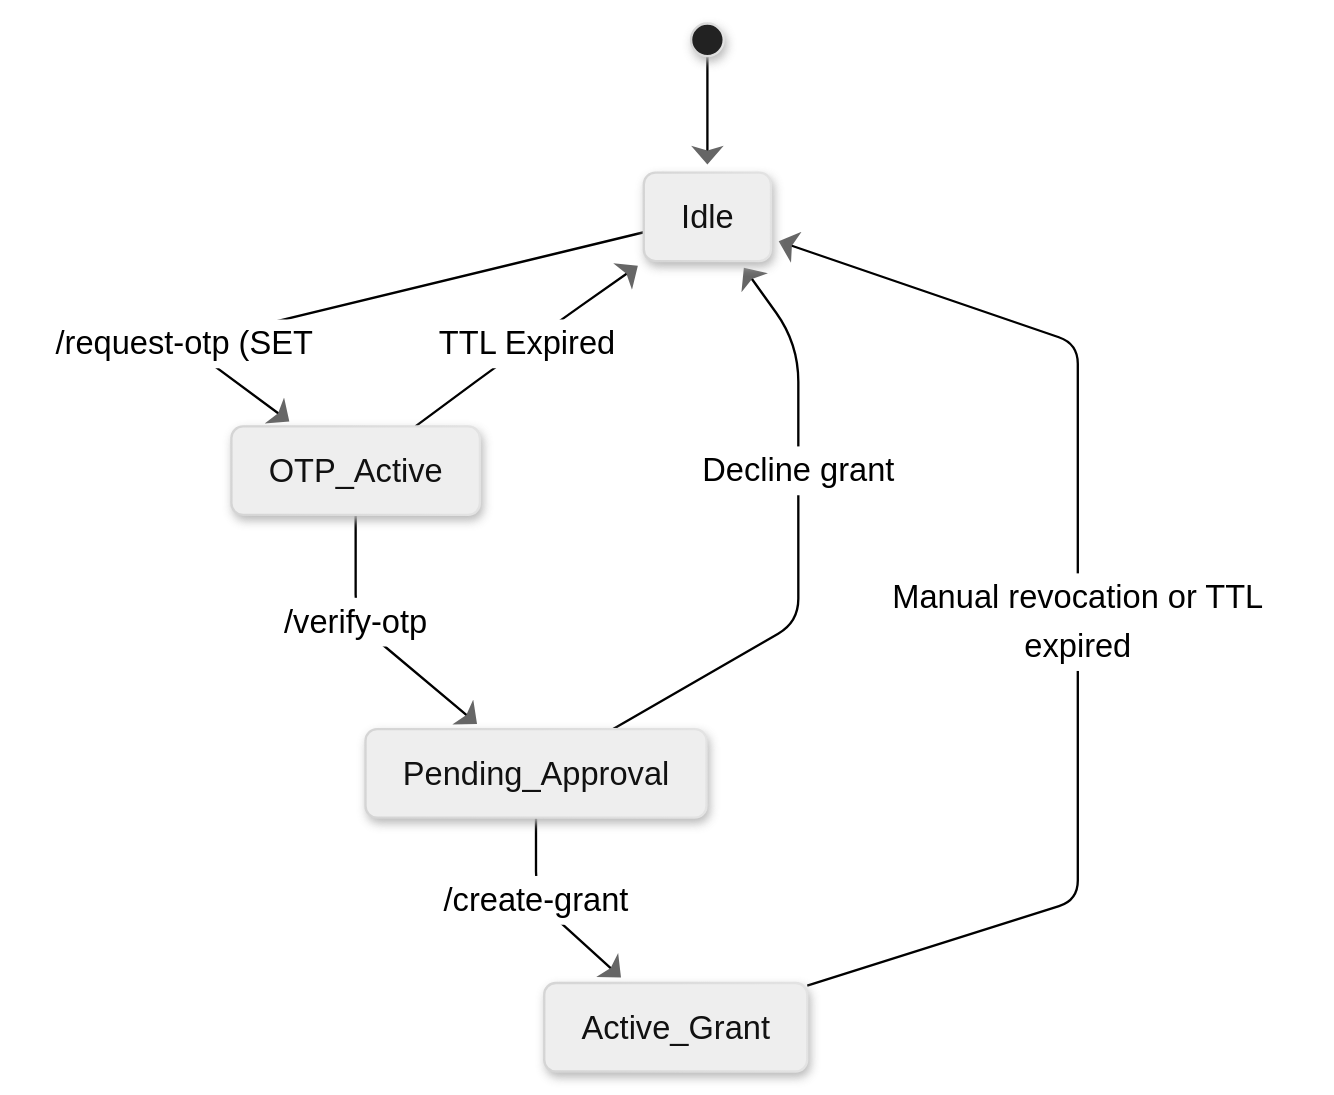
\includegraphics[width=0.85\linewidth]{Security/images/Consent-Grant-Flow/stateDiagram.png}
    \caption{Consent Grants issuance logic state diagram}
    \label{fig:consent-endpoints}
\end{figure}


\subsubsection{State Transition and Key Lifecycle}
The security of the handshake is maintained by transitioning through specific states in the high-performance cache, as outlined in Table \ref{tab:redis-states}.

\begin{table}[H]
\centering
\begin{tabular}{|l|l|l|l|}
\hline
\textbf{State} & \textbf{Redis Key Pattern} & \textbf{TTL} & \textbf{Security Goal} \\ \hline
Active OTP & \texttt{otp:active:\{code\}} & 600s & Proof of Possession \\ \hline
Pending Grant & \texttt{pending\_grant:\{uuid\}} & 600s & Identity Linkage \\ \hline
Final Grant & \texttt{grant:\{type\}:\{reqId\}:\{patId\}} & Variable & JIT Authorization \\ \hline
\end{tabular}
\caption{Lifecycle of Consent Grant States in the Redis Persistence Layer}
\label{tab:redis-states}
\end{table}



\subsection{Dynamic \texorpdfstring{\ac{JIT}}{JIT} Consent \& Capability-Based Access Lifecycle}\label{sec:JIT-lifecycle}

A core innovation of the CFI-Care platform is the dynamic consent model, 
allowing patients to delegate temporary access to their caregivers or practitioners. 
This flow is managed via a \ac{JIT} grant mechanism.

\subsubsection{Grant Mechanism}
Consent grants are stored in the primary database with an associated TTL (Time-to-Live). 
To ensure high performance, active grants are cached in Redis. 
The BFF verifies the existence and validity of these grants before forwarding patient data access requests to the FHIR server.

\subsubsection{Lifecycle Stages}
The following sequence (Figures \ref{fig:consent-part1} through \ref{fig:consent-part4}) illustrates the complete lifecycle: from the initial grant issuance to the practitioner's access, and finally, the patient-initiated revocation.

\begin{figure}[H]
    \centering
    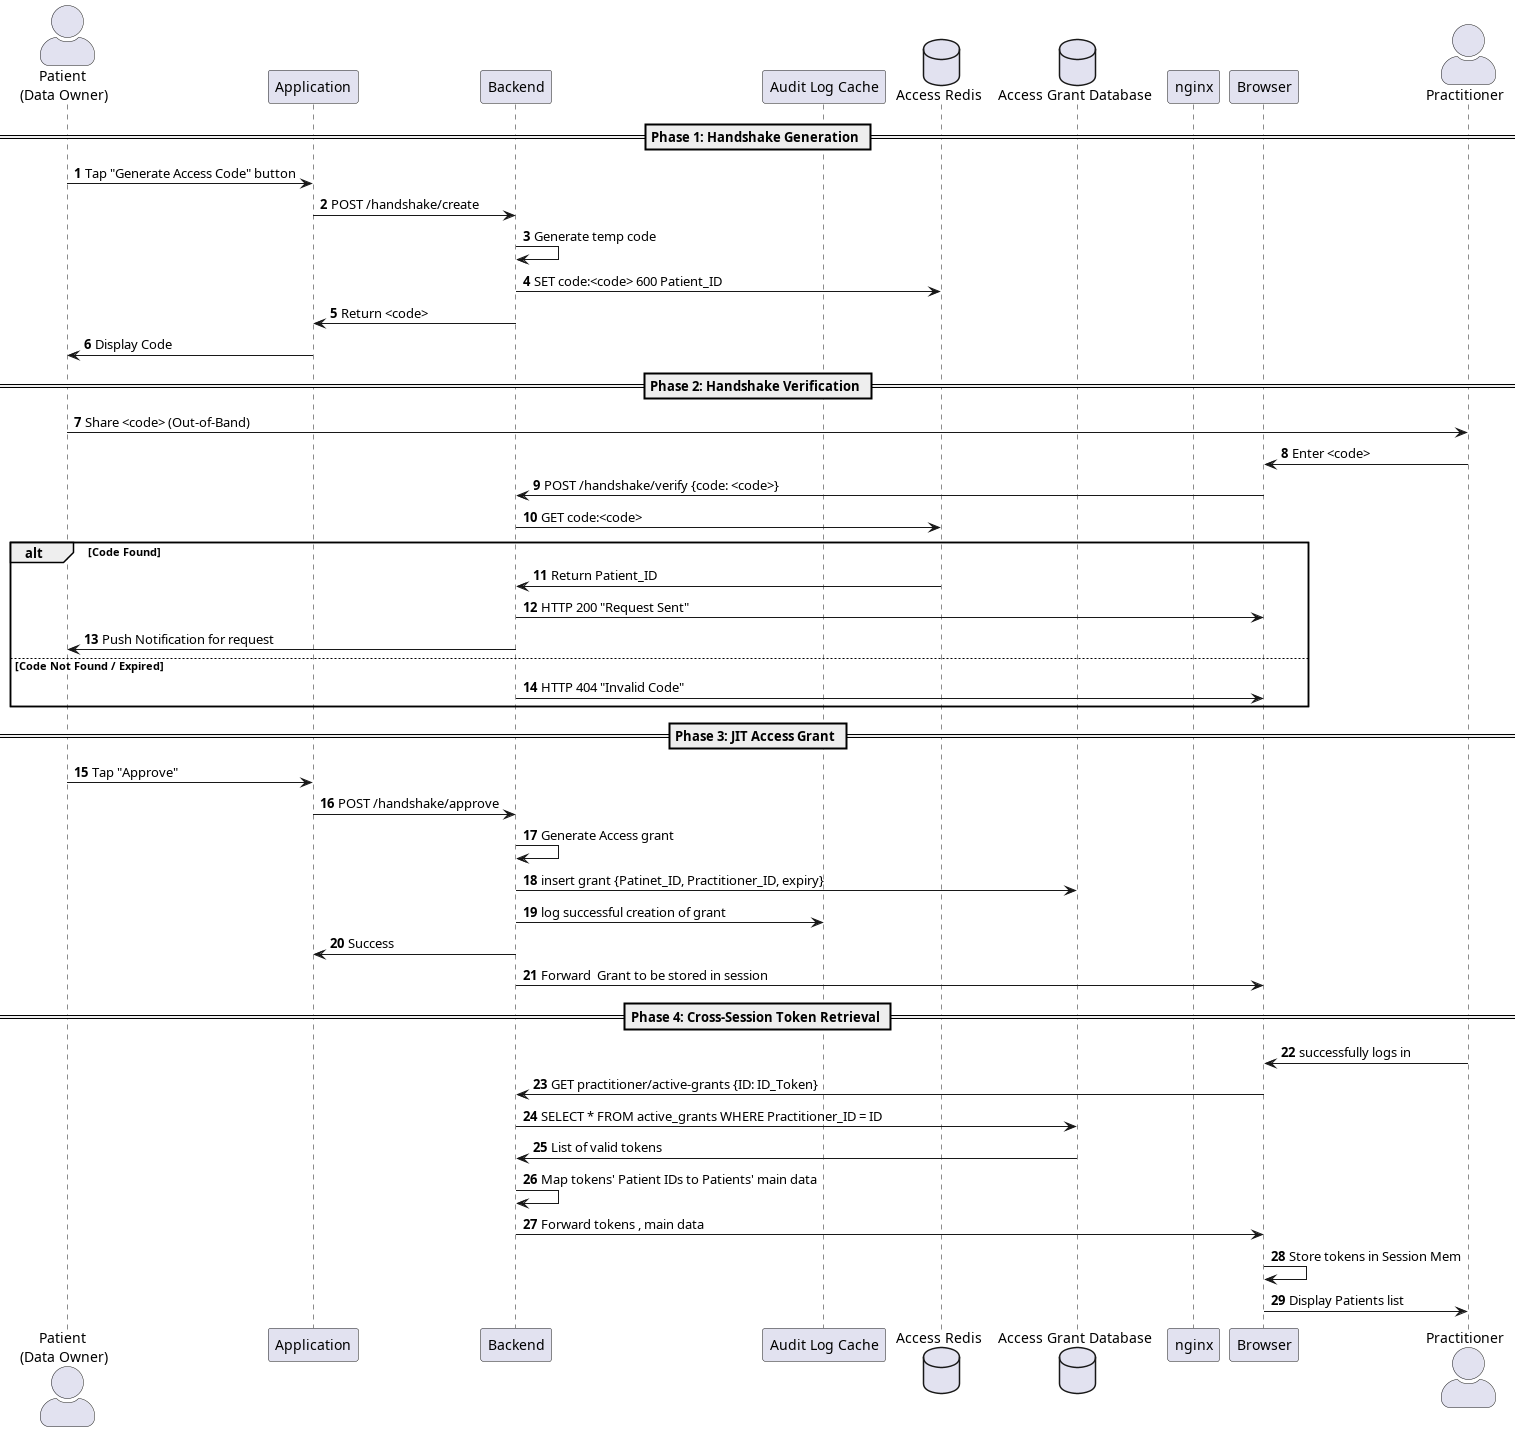
\includegraphics[width=0.9\linewidth]{Security/images/Consent-Grant-Flow/Consent-Part1/Consent-Part1.png}
    \caption{Consent Lifecycle Part 1: Patient granting access to a practitioner.}
    \label{fig:consent-part1}
\end{figure}

\begin{figure}[H]
    \centering
    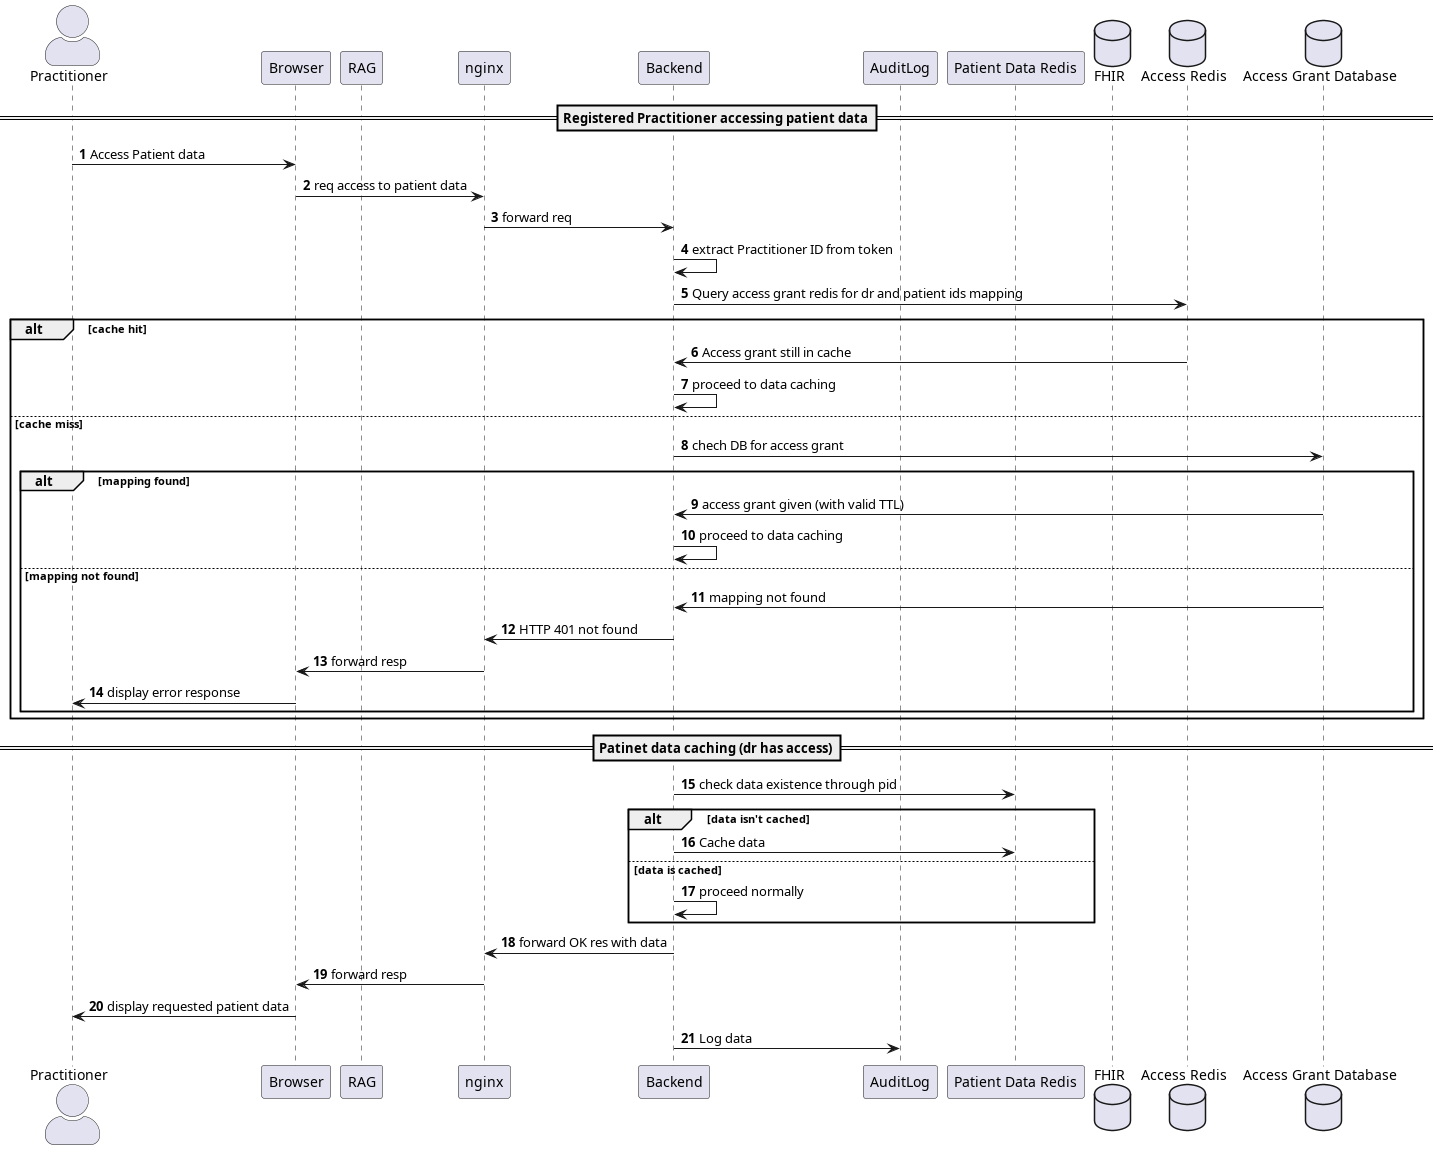
\includegraphics[width=0.8\linewidth]{Security/images/Consent-Grant-Flow/Consent-Part2/Consent-Part2.png}
    \caption{Consent Lifecycle Part 2: Practitioner accessing authorized patient data.}
    \label{fig:consent-part2}
\end{figure}

\begin{figure}[H]
    \centering
    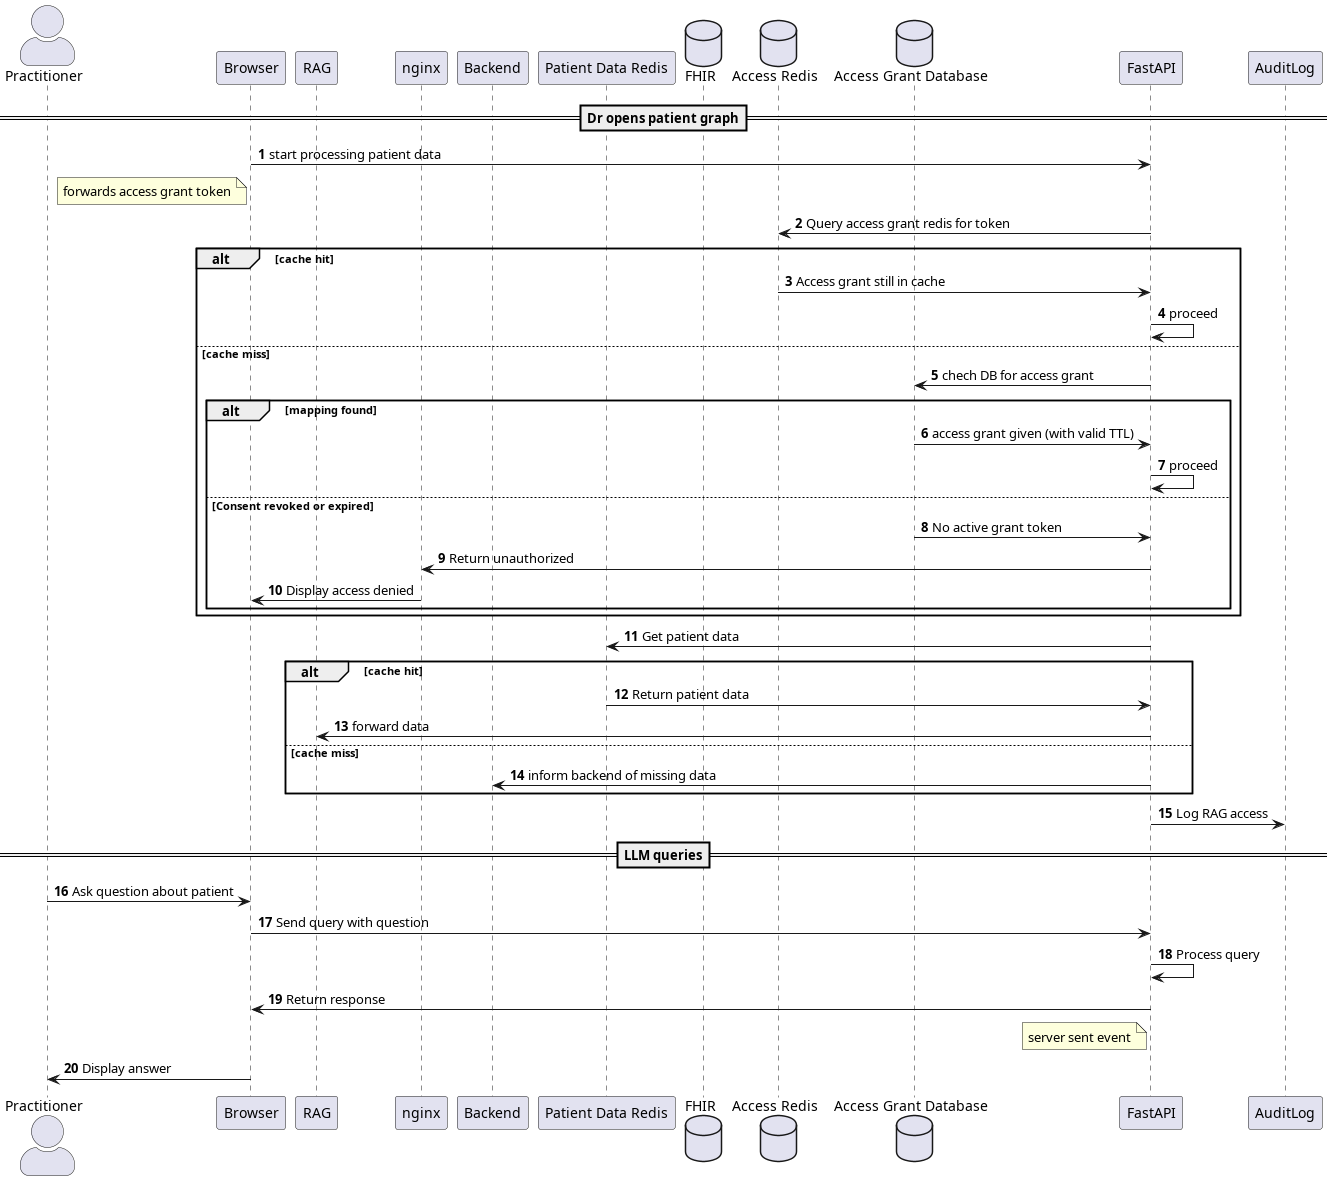
\includegraphics[width=0.8\linewidth]{Security/images/Consent-Grant-Flow/Consent-Part3/Consent-Part3.png}
    \caption{Consent Lifecycle Part 3: Patient verifying their own data access.}
    \label{fig:consent-part3}
\end{figure}

\begin{figure}[H]
    \centering
    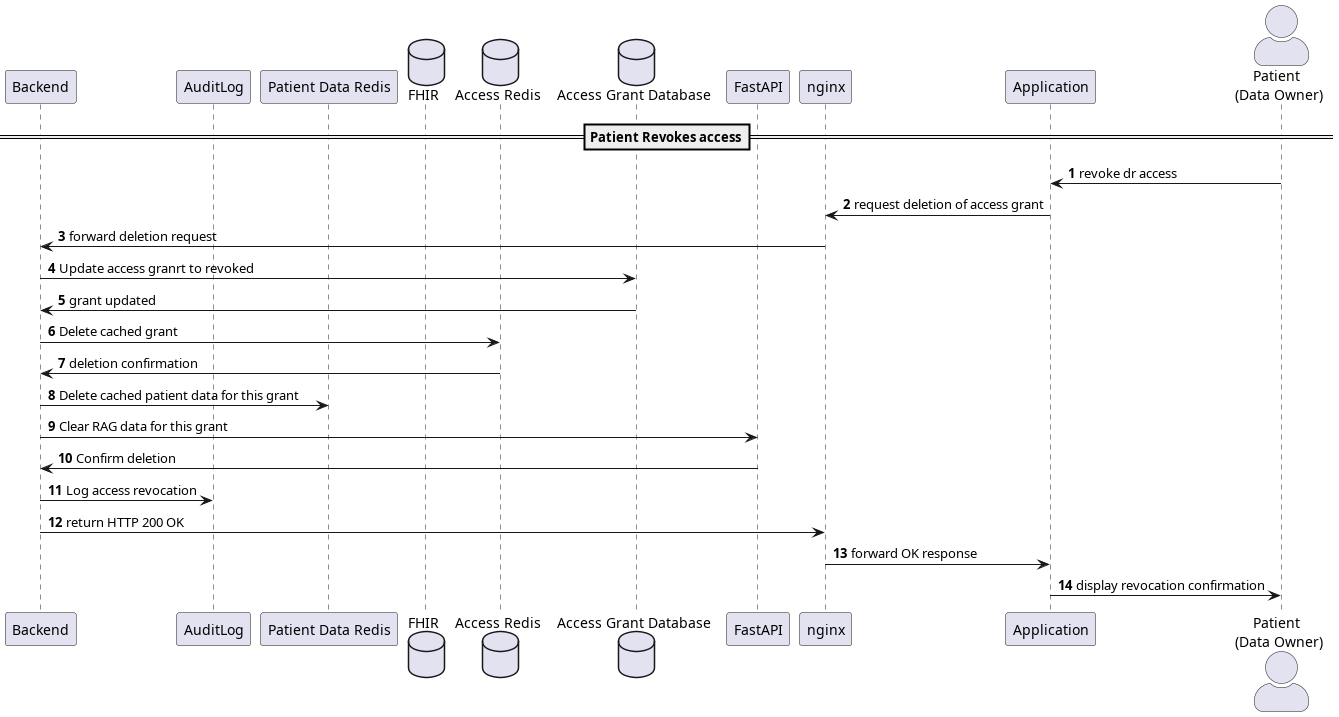
\includegraphics[width=0.85\linewidth]{Security/images/Consent-Grant-Flow/Consent-Part4/Consent-Part4.png}
    \caption{Consent Lifecycle Part 4: Patient-initiated revocation of access.}
    \label{fig:consent-part4}
\end{figure}

\paragraph{Caregiver Access}
Caregiver access follows the same patient-approved JIT consent lifecycle as practitioner access, but the caregiver identity is associated with a dedicated Keycloak \textit{Caregiver} role that is dynamically assigned
, allowing the backend to distinguish caregiver-scoped requests from ordinary patient or practitioner access. 
Once the patient approves the grant, the caregiver inherits the corresponding access level for the configured duration, subject to the same expiry and revocation checks as practitioner delegated users.
The sequence in Figure~\ref{fig:caregiver-consent} focuses on the discrepancies between caregiver and practitioner considering caregivers require context switching in the application.

\begin{figure}[H]
\centering
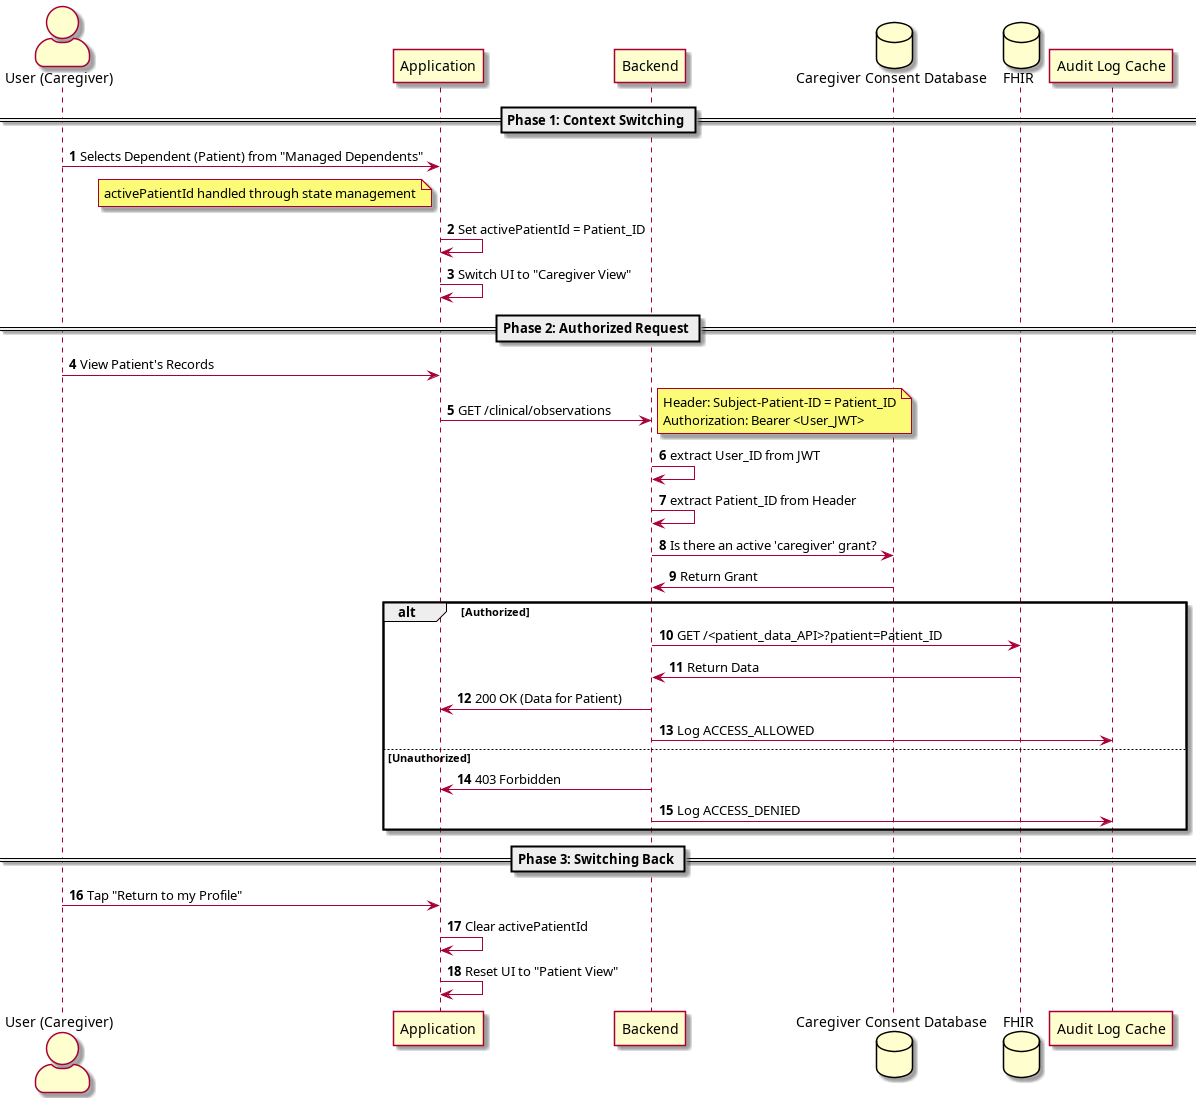
\includegraphics[width=0.85\linewidth]{Security/images/Consent-Grant-Flow/Caregiver Context Switching & Delegation.png}
\caption{Caregiver consent and JIT grant lifecycle (patient issues a transient grant to a caregiver)}
\label{fig:caregiver-consent}
\end{figure}


\subsection{State Management and Auditing}\label{sec:state-management-and-audit}

The system leverages \textbf{Redis} as a distributed state and auditing layer, ensuring that security-sensitive data is handled with atomic precision.

\begin{itemize}
    \item \textbf{Session Store:} Backs the \texttt{express-session} middleware, persisting tokens and expiration metadata.
    \item \textbf{Audit Store:} Persists security events (e.g \texttt{GRANT\_ISSUED}, \texttt{LOGIN\_FAILURE}) as sorted sets. Each entry includes metadata such as IP addresses and User-Agents, retained for 90 days to satisfy non-repudiation and privacy compliance requirements.
    % \item \textbf{Atomic Security primitives:} Redis atomic operations are used during sensitive operations to prevent race conditions, for example, OTP invalidation utilizes \texttt{GETDEL} command, which implements a "Burn-on-Read" policy, to ensure that an OTP is invalidated during the same operation it's verified, this eliminates the \ac{TOCTOU} race condition, it also eliminates the window of opportunity for replay attacks.
    
\end{itemize}

\subsubsection{Design Rationale}

% Custom OTPs are used instead of a simpler, more obvious solution like using patient's `IAM IDs' (IDs issued and stored in our IAM service, Keycloak, then used to reference patients in FHIR) directly to find and request delegated access,
% because IAM IDs are too long which makes them complex for copying into an input field, more importantly that would mean patients' IDs used across the system would need to be exposed which is a point of concern, as that allows attackers to guess valid IDs based on ID patterns
% So, using short-lived OTPs reduces the attack surface considerably, prevents User Enumeration and \ac{PII} Discovery (An attacker can't guess or confirm valid users in the system if the only provided info is a transient, random numerical code as opposed to having access to IDs whose pattern could be guessed) while maintaining system usability for users.  


Custom OTPs are used instead of exposing internal IAM IDs (Keycloak UUIDs) which are also used as FHIR resource identifiers. 
This architectural choice serves as a form of Identifier Abstraction as IAM IDs are too long, which makes them complex for manual input, and follow predictable patterns, which attackers could utilize to guess valid IDs,
in other words, exposing them at the edge would facilitate User Enumeration and \ac{PII} Discovery. 
By utilizing high-entropy, short-lived numerical OTPs, the system reduces the attack surface and limits the window of misuse while maintaining clinical usability.




% \subsubsection{BFF Middleware: Session Check, JWT Verification, Scope Validation}
% \begin{itemize}
%     \item \textbf{API auth routing}: Bearer-only enforcement: Requests without a bearer token are rejected with 401.
%     \item \textbf{Session handling}: creates/updates a BFF session record for user context and global logout coordination, based on headers from nginx,\texttt{oauth2-proxy},it's not the primary authorization mechanism
%     \item \textbf{Provisioning caller restriction}: for provisioning endpoint calls, the BFF only accepts service tokens where \texttt{client\_id} is equivalent to \texttt{KC\_PROVISIONER\_CLIENT\_ID} defined and securely stored for backend access.
%     \item \textbf{JWT verification}: validates JWT signatures against Keycloak's JWKS endpoint, checks issuer (iss), allowed audiences (aud), algorithm (RS256), and clock skew tolerance.
%           The Authorization header is forwarded by nginx as \texttt{Bearer <access\_token>} from \texttt{oauth2-proxy} auth results.
%     \item \textbf{Scope checks}: parses \texttt{scope} claim and \\ \texttt{realm\_access.roles} from the token. Compares required SMART on FHIR scopes (e.g., \texttt{patient/<id>.rs}) against token scopes using pattern matching.
%           For patient-specific scopes, validates that the \texttt{patient} claim in the token matches the requested resource ID.
% \end{itemize}

% \subsection{Doctor-Patient Consent Grants}
% The intended model supports patient-granted access for doctors, with grants
% stored in a database (grant key, scopes, TTL) Consent grants are cached in redis
% after access for performance but the databae is the main source The BFF
% verifies an active grant before calling FHIR for doctor requests. Future work:
% finalize consent persistence, and enforce patient binding in scope validation

% \begin{figure}[H]
%     \centering
%     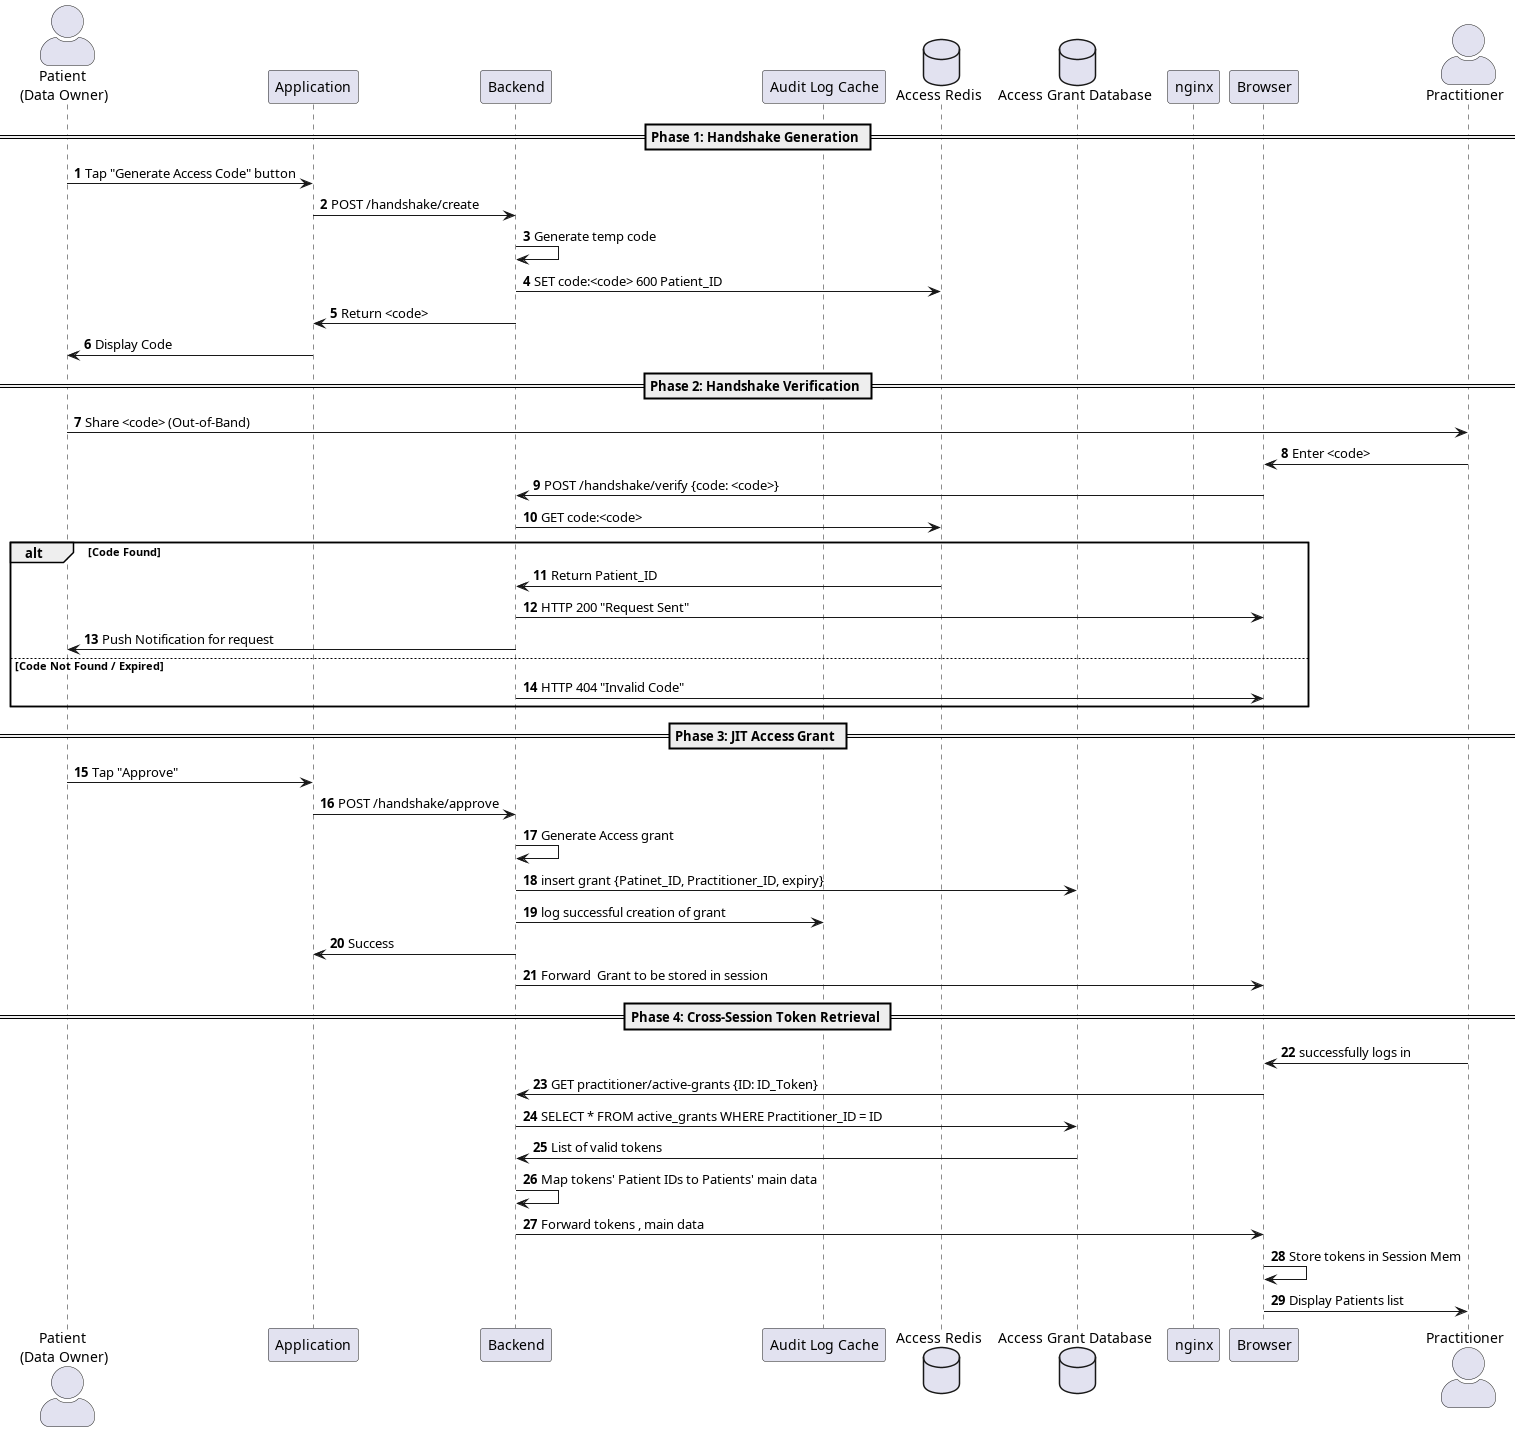
\includegraphics[width=0.85\linewidth]{Security/images/Consent-Grant-Flow/Consent-Part1/Consent-Part1.png}
%     \caption{Patients grant doctors access to their data with TTL-based revocation}
%     \label{fig:doctor-patient-access first part}
% \end{figure}
% \begin{figure}[H]
%     \centering
%     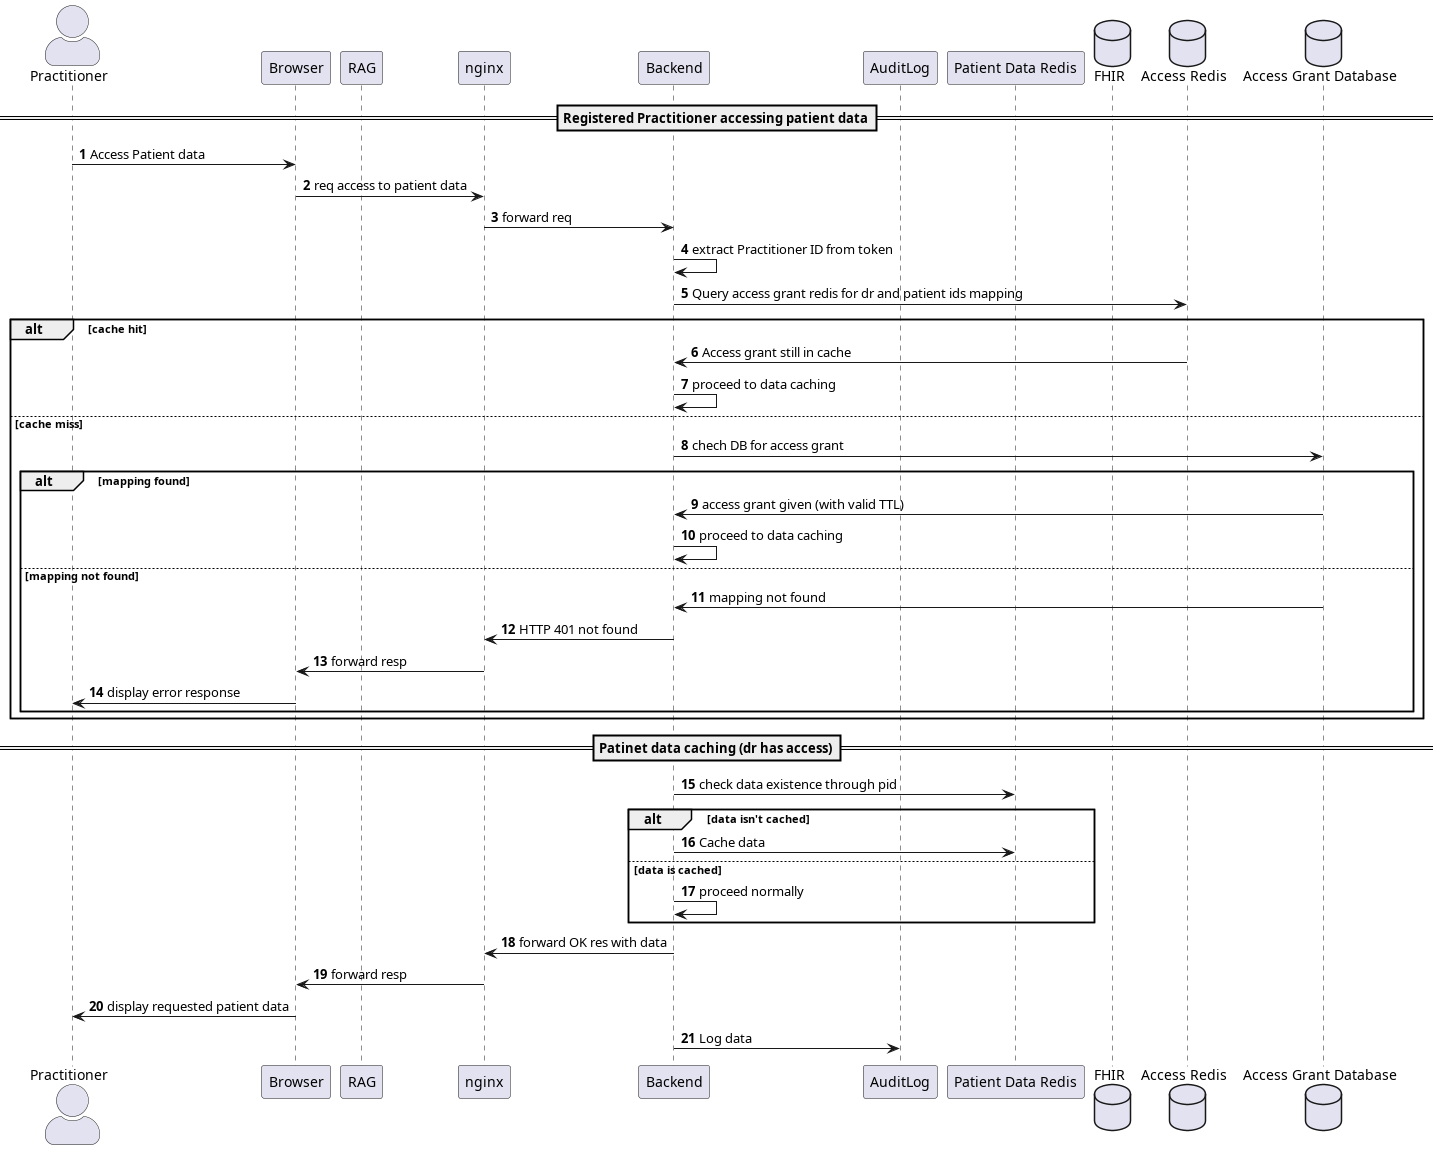
\includegraphics[width=0.85\linewidth]{Security/images/Consent-Grant-Flow/Consent-Part2/Consent-Part2.png}
%     \caption{Practitioner accessing data}
%     \label{fig:doctor-patient-access second part}
% \end{figure}
% \begin{figure}[H]
%     \centering
%     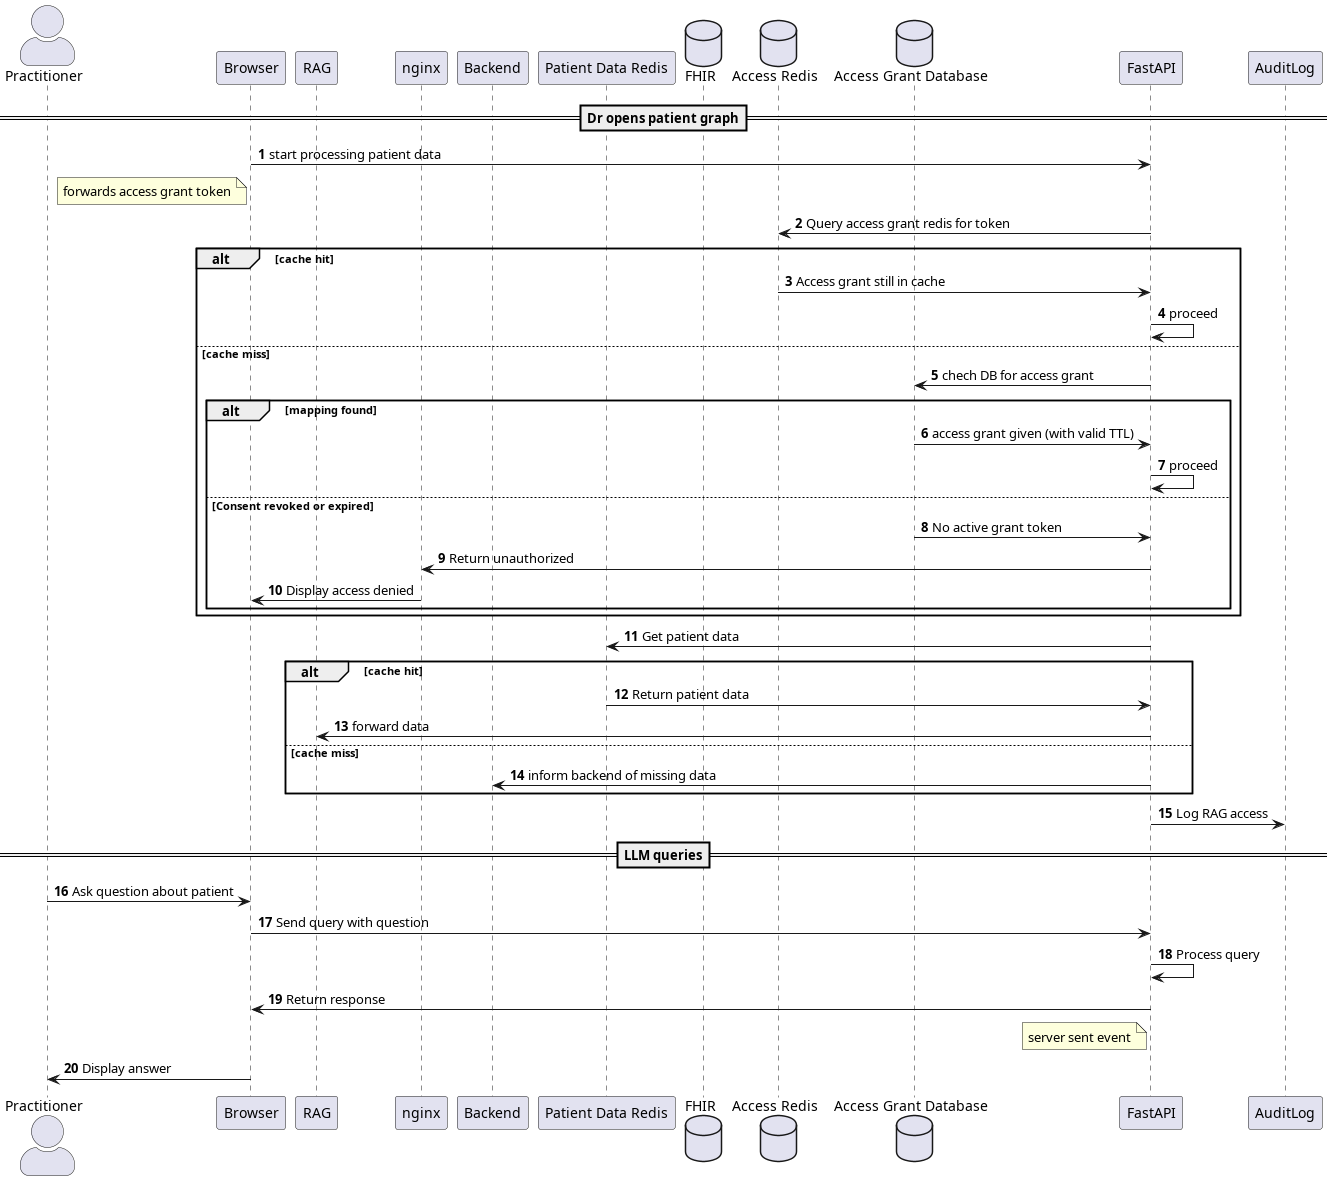
\includegraphics[width=0.85\linewidth]{Security/images/Consent-Grant-Flow/Consent-Part3/Consent-Part3.png}
%     \caption{Patient graph access}
%     \label{fig:doctor-patient-access third part}
% \end{figure}
% \begin{figure}[H]
%     \centering
%     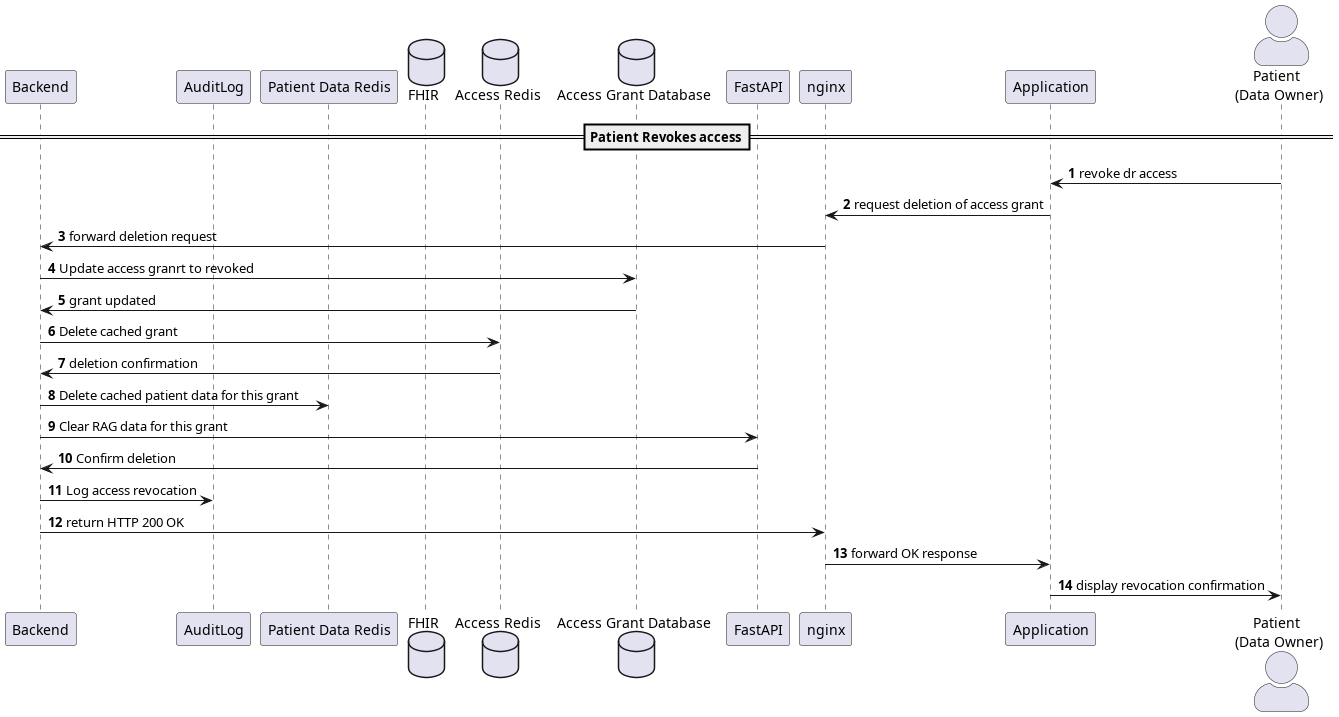
\includegraphics[width=0.85\linewidth]{Security/images/Consent-Grant-Flow/Consent-Part4/Consent-Part4.png}
%     \caption{Patient revokes grant}
%     \label{fig:doctor-patient-access fourth part}
% \end{figure}

% \subsubsection{Auditing \& Non-Repudiation}
% To ensure accountability, the Consent Grant flow implements an auditing layer. 
% Every stage of the grant lifecycle —`GRANT\_ISSUED`, `GRANT\_ACCESS\_DENIED`, and `GRANT\_REVOKED`—is logged with contextual metadata (IP, User-Agent, Timestamp, and Subject IDs), providing a full audit trail for privacy compliance.

% % \caption{Doctor-Patient Consent Granting Flow: Patients grant doctors access to their data with TTL-based revocation}

% \subsubsection{FHIR Server Enforcement}
% Future work: validate JWTs independently to implement defense in depth,
% leverage FHIR server's built-in SMART on FHIR policy enforcement for
% resource-level access control based on scopes and patient context.

% \subsubsection{JWT Verification (JWKS), Scope Checks, Patient Binding}
% JWKS-based verification validates token signatures using Keycloak's public key
% endpoint. Checks include:
% \begin{itemize}
%     \item Signature validity (RS256 algorithm).
%     \item Issuer claim (iss) matches Keycloak's realm URL.
%     \item Audience claim (aud) matches allowed audience list configured in the backend.
%     \item Clock skew tolerance configured in middleware.

% \end{itemize}

% Scope checks compare the token's \texttt{scope} claim against required route
% scopes using pattern-matching logic that handles wildcards. patient-specific
% scopes require the token's \texttt{patient} claim to match the requested
% resource Id.

% \subsection{Node.js Backend-for-Frontend (BFF) Libraries}

% \begin{itemize}
%     % \item \textbf{\texttt{express}}: HTTP server framework for handling auth, API, and health-check routes.
%     \item \textbf{\texttt{express-session} and \texttt{connect-redis}}: Server-side session storage with redis persistence, enabling stateful authentication state for browsers.
%           % \item \textbf{\texttt{joi}}: Schema validation library for login and registration input (email format, password complexity, full name pattern).
%     \item \textbf{\texttt{rate-limit-redis}}: Rate limiting middleware backed by redis. Protects endpoints from brute-force attacks.
%     \item \textbf{\texttt{jsonwebtoken}}: JWT creation and verification library %(for validation via JWKS).
%     \item \textbf{\texttt{jwks-rsa}}: Fetches and caches Keycloak's public JWKS endpoint.% Automatically refreshes keys on signature validation failure.
%     \item \textbf{\texttt{axios}}: HTTP client for outbound calls to Keycloak API.
%     \item \textbf{\texttt{helmet}}: Express middleware that sets security headers
%     \item \textbf{\texttt{cors}}: Middleware for Cross-Origin Resource Sharing, configured to accept requests from the Angular frontend origin only.
% \end{itemize}


% \subsection{Redis: Distributed State \& Session Storage}
% Two redis instances are deployed:
% \begin{itemize}
%     \item \textbf{Session Store}: backing store for express-session. Persists user sessions, access tokens, refresh tokens, and their expiration times with a 1-hour TTL.
%     \item \textbf{Audit Store}: persists authentication events (LOGIN\_SUCCESS, LOGIN\_FAILURE, REGISTER, LOGOUT, LOGOUT\_ALL) as sorted sets. Each entry includes timestamp, User ID, IP, User-Agent, and request ID. Entries expire after 90 days.
% \end{itemize}
% redis also stores user session tracking sets (all session IDs for each user) to enable logout-all operations.

% In this architecture, Redis functions as the **Primary State Store** for security-sensitive, short-lived credentials. Unlike a traditional cache, Redis is critical for enforcing the security logic of the JIT (Just-In-Time) consent flow.

% *   **Atomic Operations for Security:** The implementation utilizes atomic primitives (e.g., `set NX`, `getDel`) to prevent race conditions during OTP verification. This ensures that an OTP cannot be "replayed" or intercepted by multiple UserBs simultaneously.
% *   **Indexing with Redis Sets:** To support mobile push notifications and Granter dashboards, **Redis Sets** are used to index active handshakes. This allows for $O(1)$ complexity when adding or removing pending requests, ensuring the system remains performant as the number of users scales.
% *   **Automated Revocation via TTL:** Every security artifact—from the initial OTP to the final Grant—is bound by a TTL. This provides a "Defense-in-Depth" mechanism where access is automatically revoked even if the system fails to trigger an explicit `DELETE` command.


% \subsection{Angular Frontend Security Implementation}
% \subsubsection{Route Protection \& Guards}
% All protected routes (dashboard, med-graph/:id) are declared with \\
% \texttt{canActivate:[authGuard]}. \\ The authGuard executes before route
% activation and checks authentication status by calling the BFF's GET /auth/me
% endpoint. If the request returns \texttt{authenticated: false} or fails with
% 401, the guard navigates to the login route, where OAuth login is initiatedThis
% prevents unauthorized access to protected pages even if a user manually
% navigates via URL bar.% through \texttt{/oauth2/start}.

% \subsubsection{HTTP Interceptors \& 401 Handling}
% The global authInterceptor catches 401 responses from any API endpoint. Upon
% 401, the interceptor:
% \begin{itemize}
%     \item Logs the unauthorized attempt.
%     \item Immediately navigates to the login route (which starts oAuth via
%           \texttt{/oauth2/start}).
%     \item Re-throws the error, allowing components to also react.
% \end{itemize}
% This provides a safety net: even if a route guard passes, if the session expires during navigation, the 401 interceptor ensures the user is redirected to re-authenticate.


% \subsubsection{Reactive State Management}
% The AuthService uses a BehaviorSubject to maintain observable current user
% state. Any component can subscribe to \texttt{currentUser\$} and react to
% authentication changes.
% % \subsubsection{Error Transparency}
% % Backend validation errors (from /register endpoint) include field-level details
% % in the HTTP response's \texttt{error.details} array. The AuthService's
% % handleError method extracts and formats these messages, allowing the login
% % component to display specific guidance. This improves UX and helps users follow
% % password complexity requirements.




